\section{Results}
\label{sec:results}

\subsection{Selectivity Definitions Cluster into Two Families}
\label{sec:results:families}

Across 30 parameter configurations (11 S-score thresholds, 7 entropy
baselines, 7 Gini baselines, 5 ratio off-target indices), compound rankings
were computed for all drugs in both datasets.
Spearman correlations between the median ranking of each definition family
reveal a consistent two-cluster structure (Table~\ref{tab:correlations}).
On the Davis dataset, S-score, entropy, and Gini are mutually correlated
($r = 0.95$--$0.999$), while ratio correlates substantially less with each
($r = 0.34$--$0.46$).
On the larger Klaeger dataset, the same structure is preserved but with lower
within-cluster correlations ($r = 0.72$--$0.90$), reflecting greater
diversity of binding profiles among the 222 clinical compounds.
The ratio definition is the consistent outlier in both datasets, with
cross-family correlations of $r = 0.22$--$0.62$.

\begin{table}[h]
  \centering
  \caption{Spearman correlations between median rankings by definition family.
           Upper triangle: Davis ($n=68$). Lower triangle: Klaeger ($n=222$).}
  \label{tab:correlations}
  \begin{tabular}{lcccc}
    \toprule
                & S-score & Entropy & Gini  & Ratio \\
    \midrule
    S-score     & ---     & 0.946   & 0.952 & 0.456 \\
    Entropy     & 0.901   & ---     & 0.999 & 0.343 \\
    Gini        & 0.722   & 0.866   & ---   & 0.343 \\
    Ratio       & 0.223   & 0.483   & 0.616 & ---   \\
    \bottomrule
  \end{tabular}
\end{table}

This two-family structure reflects a fundamental difference in what the
definitions measure.
The S-score, entropy, and Gini all quantify the concentration of activity
across the full kinase panel. They differ in functional form but respond to
the same underlying property of the binding profile.
The ratio definition, by contrast, quantifies the gap between the primary
target and a specific off-target, ignoring the remainder of the binding
profile entirely.
A compound that strongly inhibits one kinase and moderately inhibits twenty
others will be ranked as highly selective by ratio (large gap to the
second target) but as moderately promiscuous by entropy and Gini
(activity distributed across many targets).

\subsection{The Two-Family Structure Replicates Across Assay Technologies}
\label{sec:results:replication}

The Davis and Klaeger pattern of Table~\ref{tab:correlations} extends to the two
further datasets, across three assay technologies and both readout types
(Figure~\ref{fig:crossdataset}).
In all four, the S-score, entropy, and Gini remain mutually correlated
(within-family Spearman $r = 0.72$--$0.999$) while the ratio definition is the
consistent outlier. Its correlation with the distribution-based family is
$0.49$--$0.56$ on the Anastassiadis functional-activity dataset and only
$0.14$--$0.19$ on the Metz $\mathrm{p}K_i$ dataset.
The degree of separation varies with the assay, but in every case the ratio
definition measures something the distribution-based definitions do not.

The instability findings also replicate.
Compounds with no active kinases (Type~1, below) are markedly more rank-unstable
than active compounds wherever such compounds exist: mean rank
$\sigma = 36.8$ vs.\ $21.7$ on Anastassiadis and $178.5$ vs.\ $108.1$ on Metz,
matching the $72.9$ vs.\ $31.3$ contrast on Klaeger (Davis contains no
zero-active compounds).
Within the distribution-based family, the number of active kinases negatively
predicts entropy instability in every dataset ($r = -0.28$ to $-0.43$), and the
top$_1$--top$_2$ affinity gap predicts ratio instability on Davis, Klaeger, and
Metz ($r = -0.44$, $-0.34$, $-0.27$; all $p < 0.001$), as detailed below.

\begin{figure}[h]
  \centering
  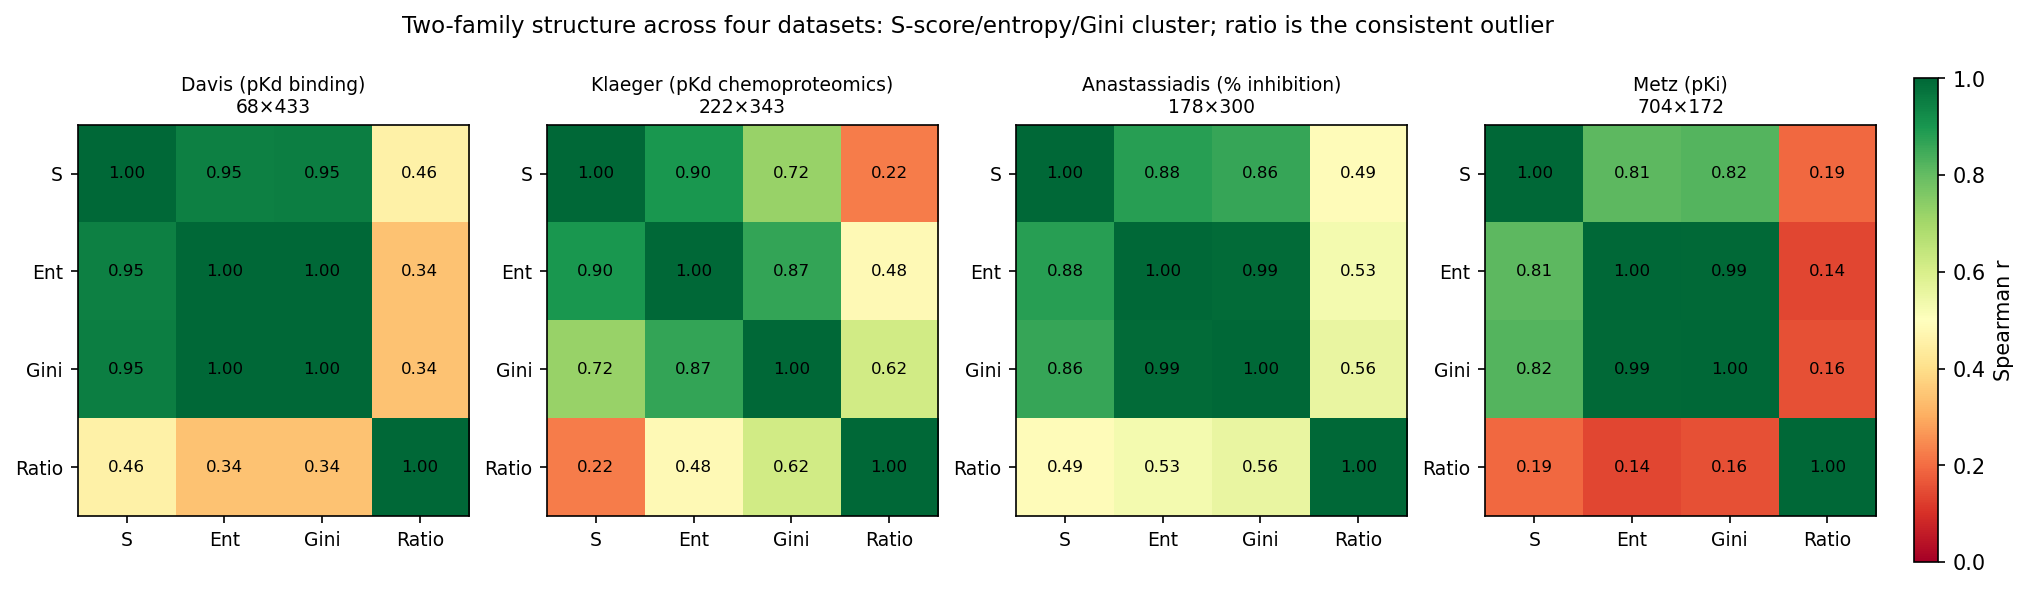
\includegraphics[width=\textwidth]{figures/cross_dataset_correlations}
  \caption{Spearman correlations between the median rankings of the
           four selectivity definitions, computed independently on each of the
           four datasets (compound $\times$ kinase panel sizes shown).
           In every dataset the S-score (S), entropy (Ent), and Gini cluster
           together while the ratio is the consistent outlier (the ratio row
           and column are the least green throughout), confirming the
           two-family structure across competition-binding, chemoproteomic, and
           functional-activity assays.}
  \label{fig:crossdataset}
\end{figure}

\subsection{Rank Instability Is Structured and Predictable}

\begin{figure}[h]
  \centering
  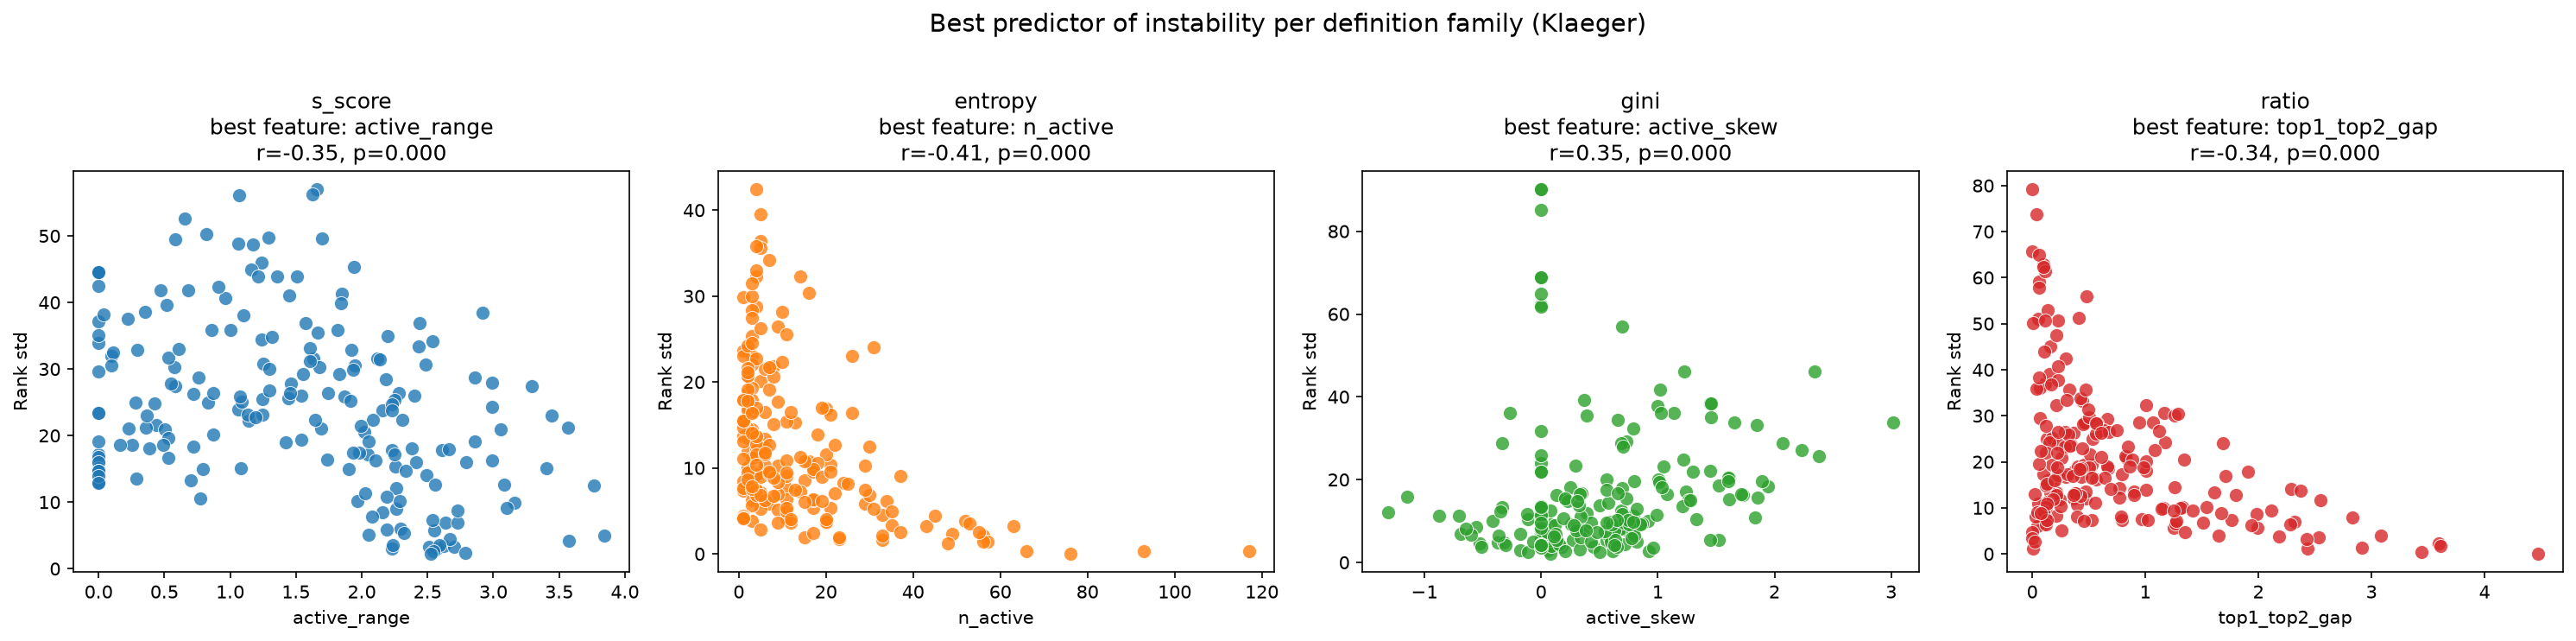
\includegraphics[width=0.85\textwidth]{figures/instability_by_family}
  \caption{Best predictor of rank instability within each definition family
           (Klaeger dataset, active compounds, $n=206$).
           Ratio instability is best predicted by the top$_1$--top$_2$ affinity gap;
           entropy, Gini, and S-score instability are best predicted by features
           of the active affinity distribution.}
  \label{fig:instability}
\end{figure}

\label{sec:results:instability}

Overall rank instability (measured as the standard deviation of a
compound's rank across all 30 configurations) varies substantially across
compounds (Klaeger: mean $\sigma = 34.3$, range $7.0$--$90.7$;
Davis: mean $\sigma = 8.5$, range $1.8$--$19.3$).
Instability is not uniformly distributed: within each definition family,
specific binding profile features predict which compounds receive unstable
rankings (Table~\ref{tab:predictors}).

Within the ratio family, the gap between the top and second-ranked affinities
(top$_1$--top$_2$ gap) is the strongest predictor of instability
(Figure~\ref{fig:instability})
($r = -0.444$, $p < 0.001$ on Davis, and $r = -0.341$, $p < 0.001$ on Klaeger).
Compounds with near-identical affinities for their two best-bound kinases
receive highly variable ratio rankings because the choice of reference
off-target ($k = 1$ vs.\ $k = 2, \ldots, 5$) determines whether the compound
appears selective or promiscuous.

Within the entropy and Gini families, the number of active kinases
($\mathrm{p}K_d > 6$) negatively predicts instability
($r = -0.279$, $p < 0.05$ for entropy on Davis,
$r = -0.409$, $p < 0.001$ on Klaeger).
Compounds with many active kinases have well-defined broad profiles whose
entropy and Gini scores are stable across baseline choices, while compounds with few
active kinases are sensitive to the baseline because small changes can move
targets in or out of the active set, altering the distribution substantially.
The active affinity range is also a significant predictor for the S-score and
entropy on Klaeger ($r = -0.35$ and $-0.27$, both $p < 0.001$). Gini is not
significantly predicted by this feature ($r = -0.10$, $p = 0.15$). It is consistent with the interpretation that heterogeneous
profiles (whose affinities span a wide range) yield more reproducible rankings
across parameter choices than flat profiles (in which many near-equal affinities
reshuffle as the parameter changes).

Gini instability's strongest 
predictor in either dataset
($r = +0.346$, $p < 0.001$ on Klaeger) is skewness, exceeding every other feature--family
pairing in Table~\ref{tab:predictors} apart from the ratio's top$_1$--top$_2$
dependence. Unlike the other features above, it
targets what Gini measures directly, i.e. the shape of
the active-affinity distribution's inequality.
The positive sign of this correlation is consistent with right-skewed active
distributions being the least stable. Most active kinases bound only modestly
above threshold, with one (or a few)
much more potent outliers, concentrating mass near the baseline boundary.
A small shift in $\beta$ moves that mass in or out of the active set.
Left-skewed profiles (most active kinases tightly bound, few sitting near
threshold) are comparatively insensitive to that choice. As with active
affinity std/range above, the relationship does not replicate on Davis
($r = +0.043$, $p = 0.73$).

Unlike the other families, the S-score's instability is significantly predicted
by every profile-shape feature except the top$_1$--top$_2$ gap
(Table~\ref{tab:predictors}), and most strongly by the spread of active
affinities. Compounds whose active affinities cluster near the threshold gain or
lose panel hits under small shifts in $\tau$, whereas those with a wide affinity
range retain a stable hit count regardless of the exact cutoff.
This S-score pattern is specific to Klaeger, however, on Davis, no profile feature
significantly predicts S-score instability (all $|r| \le 0.16$;
Table~\ref{tab:predictors}, right). A possible explanation is that a threshold
count's instability is governed by where each assay's detection window falls
relative to the cutoff, and the two assays place
that window very differently: 3.6\% of the Klaeger matrix is active versus
17.9\% of Davis (Methods). 
The one predictor that replicates cleanly across both datasets is the
ratio family's dependence on the top$_1$--top$_2$ gap (above), which compares
two affinities directly rather than counting how many pass a cutoff. The entropy
dependence on the number of active kinases replicates in direction but more
weakly on the smaller Davis panel ($r = -0.409$ on Klaeger vs.\ $-0.279$ on
Davis). Gini shows the reverse pattern in strength, reaching significance on
Davis ($r = -0.300$) but not on Klaeger ($r = -0.093$).

\begin{table}[h]
  \centering
  \caption{Spearman correlations between binding profile features and
           within-family rank instability, on the Klaeger ($n=206$ active drugs)
           and Davis ($n=68$) datasets. Columns are the S-score (S), entropy (E),
           Gini (G), and ratio (R) families. The ratio family's dependence on the
           top$_1$--top$_2$ gap replicates strongly on both datasets. The
           S-score's dependence on the active-affinity spread does not (no feature
           is significant on Davis), and neither does Gini's dependence on
           active-affinity skew. Significance:
           * $p<0.05$, ** $p<0.01$, *** $p<0.001$.}
  \label{tab:predictors}
  \resizebox{\textwidth}{!}{%
  \begin{tabular}{lcccc@{\hskip 1.4em}cccc}
    \toprule
    & \multicolumn{4}{c}{Klaeger ($n=206$)} & \multicolumn{4}{c}{Davis ($n=68$)} \\
    \cmidrule(lr){2-5}\cmidrule(lr){6-9}
    Feature & S & E & G & R & S & E & G & R \\
    \midrule
    $n_\mathrm{active}$      & $-0.272^{***}$ & $-0.409^{***}$ & $-0.093$       & $-0.040$       & $-0.153$ & $-0.279^{*}$ & $-0.300^{*}$ & $+0.294^{*}$ \\
    top$_1$--top$_2$ gap     & $+0.039$       & $+0.082$       & $+0.031$       & $-0.341^{***}$ & $-0.079$ & $-0.007$     & $-0.029$     & $-0.444^{***}$ \\
    Active affinity std      & $-0.281^{***}$ & $-0.170^{*}$   & $-0.117$       & $-0.107$       & $+0.009$ & $-0.015$     & $+0.005$     & $+0.040$ \\
    Active affinity range    & $-0.354^{***}$ & $-0.273^{***}$ & $-0.102$       & $-0.116$       & $+0.011$ & $-0.111$     & $-0.098$     & $+0.134$ \\
    top$_2$ $\mathrm{p}K_d$  & $-0.314^{***}$ & $-0.234^{***}$ & $-0.192^{**}$  & $+0.186^{**}$  & $-0.055$ & $-0.203$     & $-0.187$     & $+0.296^{*}$ \\
    Active affinity skew     & $-0.162^{*}$   & $-0.045$       & $+0.346^{***}$ & $-0.108$       & $+0.026$ & $+0.066$     & $+0.043$     & $+0.069$ \\
    \bottomrule
  \end{tabular}%
  }
\end{table}

Five additional candidates features were tested:
two concentration measures from industrial-organization
economics ((1) the top-target concentration ratio (CR$_1$) and (2) the
Herfindahl--Hirschman Index (HHI)). These were sourced from the same 
field as the Gini coefficient \cite{Graczyk2010}. We also tested
(3) the raw
primary-target affinity (top$_1$ $\mathrm{p}K_d$), (4) a near-tie count
generalizing the top$_1$--top$_2$ gap, and (5) the active-affinity coefficient of
variation. CR$_1$ and HHI turned out to be near-collinear with
$n_\mathrm{active}$, which is already in the table ($r = -0.98$ to $-0.99$ and $-0.998$,
respectively, on both datasets). The
remaining three were uniformly weaker predictors than the features already
included, in every family and both datasets (full numbers in the code
repository).

\subsection{Three Mechanistically Distinct Sources of Instability}

\begin{figure}[h]
  \centering
  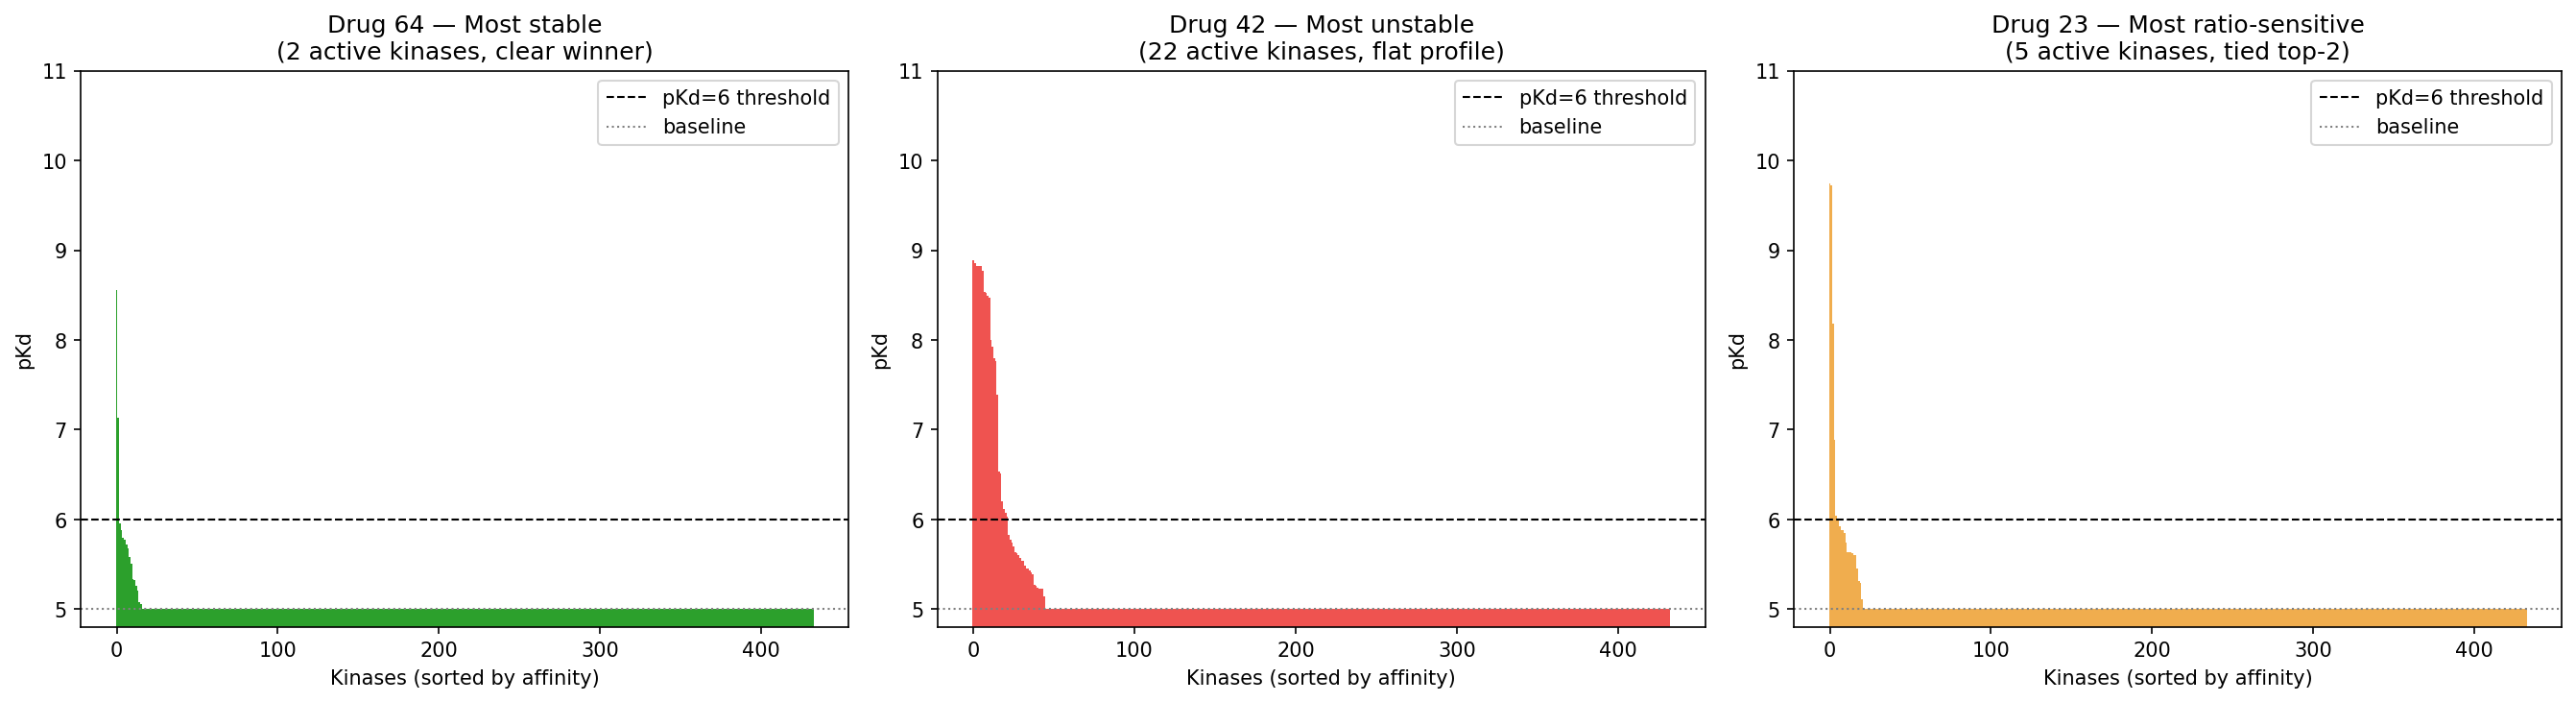
\includegraphics[width=0.85\textwidth]{figures/binding_profiles}
  \caption{Representative binding profiles illustrating the three instability types.
           Left: Drug~64 (Davis), most stable ($\sigma = 1.8$), two active kinases.
           Center: Drug~42 (Davis), most unstable ($\sigma = 19.3$), 22 active kinases
           with no dominant target.
           Right: Drug~23 (Davis), most ratio-sensitive, five active kinases
           including two near-tied top targets ($\Delta\mathrm{p}K_d = 0.023$).
           Dashed line: $\mathrm{p}K_d = 6$ activity threshold;
           dotted line: $\mathrm{p}K_d = 5$ assay floor.}
  \label{fig:profiles}
\end{figure}

\label{sec:results:taxonomy}

Examination of the most and least unstable compounds in the Klaeger dataset
reveals three structurally distinct sources of rank instability
(Figure~\ref{fig:profiles}), each
implicating a different aspect of how the definitions are constructed.

\textbf{Type~1: Zero-active compounds.}
The five most unstable Klaeger compounds (AZD-8055, BMS-911543, Vatalanib,
Filgotinib, ARRY-380; rank $\sigma > 76$) all have zero active kinases at the
$\mathrm{p}K_d > 6$ threshold.
These compounds have no meaningful binding to any profiled kinase at
sub-micromolar affinity, yet all four definitions still assign them numerical
selectivity scores based on the detection floor values.
The resulting rankings are arbitrary: different parameterizations produce
different orderings of compounds that are, in practice,
indistinguishable from one another.
Mean rank instability for zero-active compounds is $\sigma \approx 73$,
compared with $\sigma \approx 31$ for compounds with at least one active
kinase ($p < 0.001$, Mann--Whitney $U$ test).
Davis has no such compounds at all: every Davis compound
has at least one active kinase, consistent with Davis's fixed-concentration
screening design, which reports a $K_d$ only when activity is first detected
at 10~$\mu$M. The same zero-active instability contrast reported here for
Klaeger also holds on the two further datasets in
Section~\ref{sec:results:replication}.

\textbf{Type~2: Near-tied top targets.}
When an active compound's two best-bound kinases have near-identical affinities, the
ratio is highly sensitive to which is designated the primary target and which
the reference off-target, because a small parameter change can swap their roles
(the top$_1$--top$_2$ gap is the strongest predictor of ratio instability, above).
Drug~23 in the Davis dataset (top$_1$--top$_2$ gap $= 0.023$~pKd units) is the
extreme case: its two best-bound kinases are essentially indistinguishable, so
it receives maximally unstable ratio rankings.

\textbf{Type~3: Broad profiles with a dominant primary target.}
The largest entropy-ratio disagreements in the Klaeger dataset arise for
compounds with high $n_\mathrm{active}$ and a large top$_1$--top$_2$ gap
(e.g.\ Dovitinib: $n_\mathrm{active} = 26$, gap $= 1.935$;
BMS-690514: $n_\mathrm{active} = 20$, gap $= 1.985$).
These compounds have one clearly dominant target but also bind many kinases at
moderate affinity.
The ratio definition scores them as highly selective (large gap between primary
and secondary target), while the entropy and Gini definitions score them as
moderately promiscuous (activity spread across many targets).
Neither characterization is incorrect, as they reflect genuinely different
questions about selectivity. 

Conversely, the most stable compounds in both datasets (e.g.\ XL-228,
$\sigma = 7.0$; PF-03814735, $\sigma = 7.8$) are highly promiscuous, with
55--57 active kinases.
When a compound binds nearly the entire profiled kinome, all definitions rank
it as non-selective regardless of parameterization, producing low instability.

\subsection{Panel Size Dependence of Selectivity Rankings}
\label{sec:results:panelsize}

To assess the stability of selectivity rankings as a function of kinase panel
size, we performed a subsampling analysis on the two datasets with genuine
sparse kinase coverage: Klaeger (343 kinases, chemoproteomic dose--response
profiling) and Metz (172 kinases, a medicinal-chemistry campaign), in each of
which compounds were tested against only a subset of the panel.
The Davis and Anastassiadis datasets were not used for this analysis, because
both are dense complete-matrix screens (every compound tested against every
kinase by construction) rather than the sparse coverage of real profiling
panels. Subsampling their kinases would also change the apparent number of
active compounds in ways that confound the panel size effect with the
zero-active instability characterized in the instability taxonomy above.

For each panel size (Klaeger $p \in \{50, 80, \ldots, 320, 343\}$; Metz
$p \in \{50, 80, \ldots, 170, 172\}$), we drew 50 random subsets of $p$ kinases
from the full panel, computed each selectivity definition on the subpanel, and
measured agreement with the full-panel ranking using Spearman correlation.
We call a panel size ``recovering'' the full-panel ranking once this mean
correlation exceeds $0.90$, adopting the same numerical bar reliability
conventionally sufficient to call a measurement ``excellent'' \cite{Koo2016}. 
Altering the choice of correlation cutoff changes the reported $p^*$ values,
however, the
ratio definition remains the slowest to recover and the Gini coefficient the
second-slowest for any bar between $0.80$ and $0.95$. Only the relative order
of entropy and the S-score is bar-dependent within this range (full numbers
in the code repository).

On Klaeger, the four definitions differ substantially in their panel size
requirements (Figure~\ref{fig:panelsize}).
Selectivity entropy and the S-score both reach mean $r = 0.90$ against the
full-panel ranking at approximately 110 kinases.
The Gini coefficient requires approximately 290 kinases to reach the same
threshold.
The ratio definition does not reach $r = 0.90$ at any subpanel size short of
the full panel: it achieves only $r = 0.888$ even at 320 kinases, just 23
below the full panel of 343, and attains $r = 0.90$ only on the complete panel.

This result has a direct practical implication.
Standard commercial kinase selectivity panels typically profile 50--100
kinases.\cite{Bosc2017}
At these panel sizes, entropy- and S-score-based rankings are reasonably
stable ($r \approx 0.76$--$0.85$), but Gini and ratio rankings are effectively
uncorrelated with what would be obtained on a full kinome panel
($r < 0.14$ for Gini, $r < 0.00$ for ratio at $p = 50$).
Ratio rankings in particular are unreliable at any panel size commonly used
in practice, because the identity of the reference off-target ($k$-th ranked
kinase) changes substantially as panel composition changes.

To test whether these patterns generalize beyond a single assay, we repeated the
analysis on Metz (172 kinases; Figure~\ref{fig:panelsize}, right). The ordering
of the definitions by panel-size requirement is preserved. The distribution-based
definitions recover the full-panel ranking from a small fraction of the panel
(S-score at approximately 50 kinases, entropy and Gini at approximately 80),
while the ratio again lags, reaching $r = 0.90$ only at 170 of the 172 kinases.
We note that the ratio's poor recoverability is universal, holding
on both sparse datasets, which strengthens the case that it measures a distinct,
panel-composition-dependent property. We also note that the Gini coefficient is the one
measure whose recoverability is dataset-specific. It is slow on Klaeger ($p^* = 290$),
but fast on Metz ($p^* = 80$), so its poor behavior on Klaeger should not be read
as a general property. Entropy and the S-score are fast on both.

\begin{figure}[h]
  \centering
  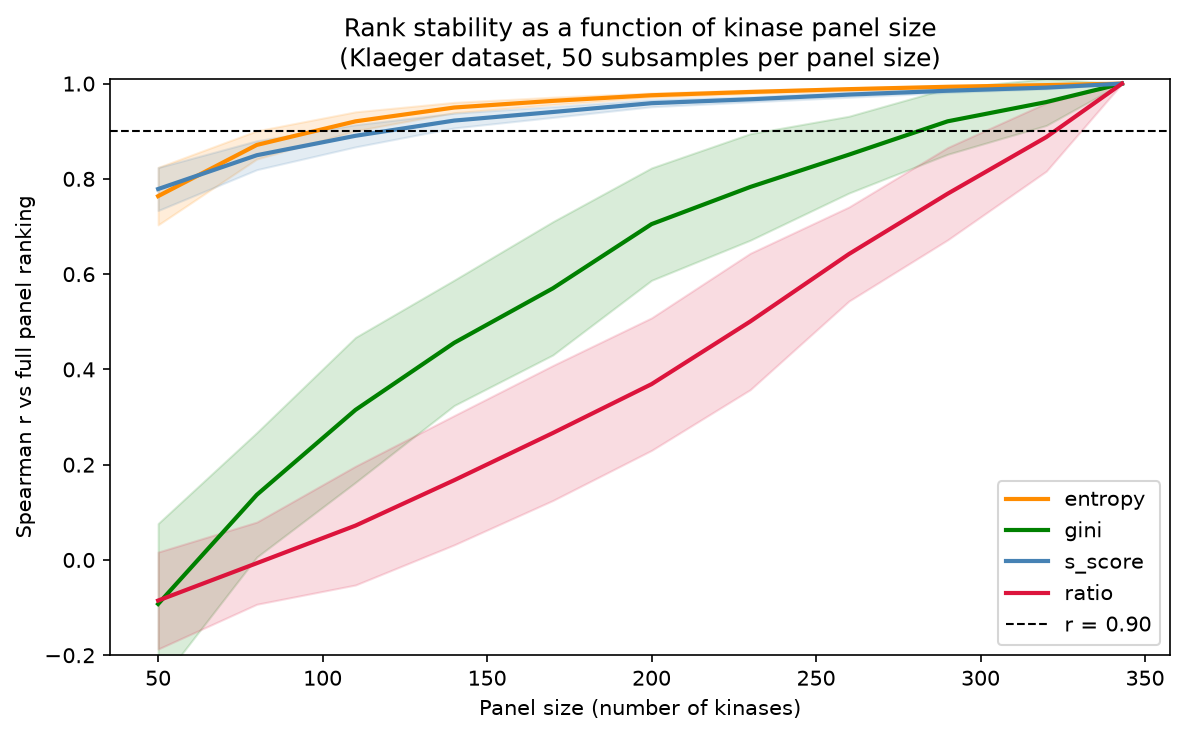
\includegraphics[width=\textwidth]{figures/panel_size_stability}
  \caption{Mean Spearman correlation between rankings computed on random kinase
           subpanels and rankings on the full panel, as a function of subpanel
           size, for the two sparse-coverage datasets: Klaeger (left, 343 kinases)
           and Metz (right, 172 kinases).
           Shaded bands indicate $\pm 1$ standard deviation across 50 subsamples;
           the dashed line marks $r = 0.90$.}
  \label{fig:panelsize}
\end{figure}
